\subsection{Resumen}

El uso de la cache es distinto para ambos compiladores: Usando programas para ver el contenido y el uso del cache (como por ejemplo valgrind) procesaremos varias imágenes, de distintos tamaños y no cuadradas, para corroborar que de acuedo al compilador, el uso de la cache varía. Primero vamos a comparar ambos sin optimización alguna. Luego vamos a repetir los experimentos activando las optimizaciones para ambos casos. \\


\subsection{Experimentaciones de caché sin optimización}

Veremos a continuacion si el uso de la cache por ambos compiladores es igual, similar o completamente diferente. Nosotros esperamos ver que sea diferente. Para esto realizaremos varias pasadas con los filtros implementados en c a diferentes imagenes utilizando dos compiladores diferentes, ICC y GCC sin la opción para optimizar. \\

Utilizaremos el valgrind, el cual nos muestra los \textit{misses} y las prediciones de saltos fallidos, dependiendo de esos resultados podremos concluir si el uso de la cache es igual de eficiente o si varía .\\


Primero veremos como es el comportamiento con el filtro blur. Por cuestiones referentes al tiempo vamos a utilizar un radio chico ya que a medida que aumenta el radio, el emulador tiene un costo temporal demasiado elevado.Usamos en este caso radio 10 y lo que va a ir variando es el tamaño de la imagen. Si hay diferencias en el uso de la cache con radios chicos, con radios mas grandes esta diferencia se va a mantener o incluso aumentar, por eso consideramos que fijar el radio no perjudica nuestro experimento. \\

\subsection{Datos obtenidos:}

\begin{figure}[H]
\begin{center}
%\minipage{0.8\textwidth}
  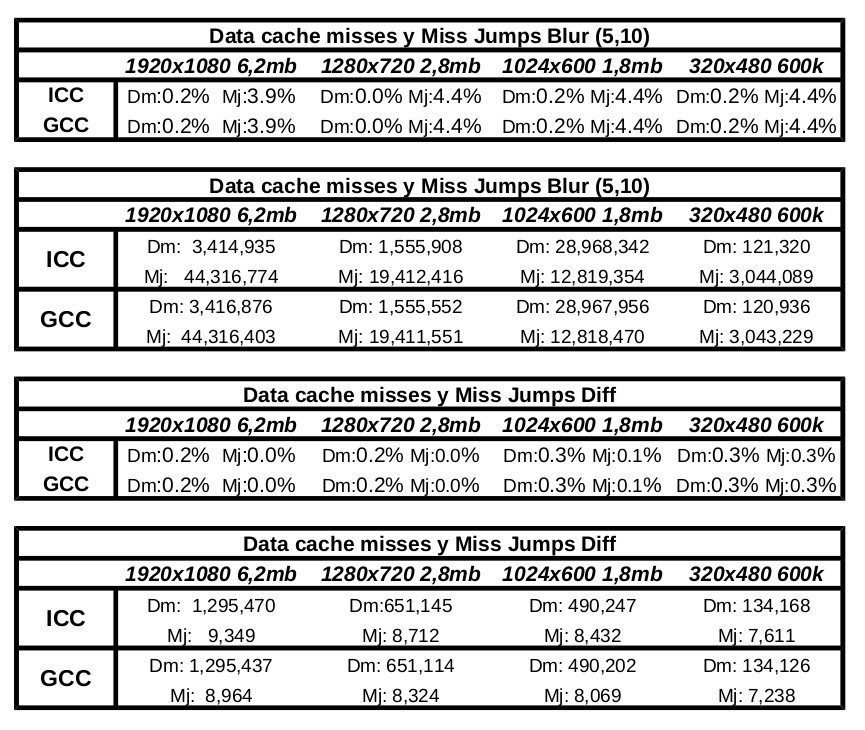
\includegraphics[width=\linewidth]{cachecompiladores/tabla.png}
%\endminipage
\end{center}
\end{figure}

\subsection{Conclusion}

Luego de obtener los resultados y analizarlos observamos que si bien los valores de misses y miss jumps son muy parecidos , no son lo suficientemente parecidos como para concluir que el uso de la cache que hacen ambos compiladores es el mismo. Esto lo deducimos porque vimos que cuando corrimos varias veces el mismo filtro a la misma imagen utilizando siempre solo un compilador, al ver los resultados (los miss cache), estos varian entre si en muy poco (+- diez ), pero si compramos los resultados de misses obtenidos utilizando compiladores diferentes estas variaciones son suficientemente grandes como para ver que definitivamente no hacen lo mismo. \\

Por otro lado si miramos los porcentajes, se observa que ambos tienen exatamente los mismos valores para cualquiera de los dos filtros, en cualquier situacion. Finalmente podemos concluir que en realidad los compiladores manejan la cache de maneras distintas al menos sin las optimizaciones activas. Como un detalle, se puede ver que ICC tiende a tener mas misses y miss jumps que GCC. Antes habiamos visto que ICC es mas rápido que GCC.


\subsection{Experimentaciónes de la caché con optimizaciones activas}

Para esta etapa del experimento vamos a activar la opción de optimización \textit{-O3} para ambos compiladores y vamos a ver como esto influye en el manejo de la memória caché.\\
Para medir ese aspecto vamos a usar la herramienta de Valgrind \textit{Cachegrind} que nos va a mostrar el valor y el porcentaje de los Miss Jumps y los Data miss.\\
 Mediante las siguientes mediciones vamos a tratar de corroborar o refutar la hipotesis de que ambos compiladores manejan la moria caché de una manera distinta.\\
En particular, teniendo en cuenta el experimento realizado anteriormente en el que vimos la ventaja en cuanto al tiempo del ICC sobre el GCC, esperamos ver un mejor manejo también en este aspecto a favor del compilador ICC.\\
Nota: Las imágenes usadas para estas mediciones fueron las siguientes:\\
320x480: 480.bmp\\
512x512: azul24.bmp\\
800x600: scene0.bmp\\
1920x1080: 1k.bmp \\


\subsection{Datos obtenidos:}

\begin{figure}[H]
\begin{center}
%\minipage{0.8\textwidth}
  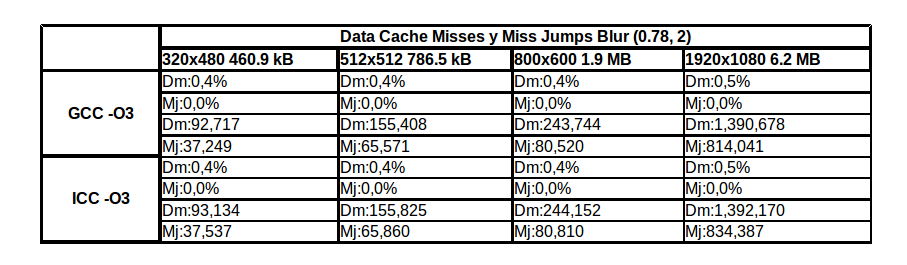
\includegraphics[width=\linewidth]{cachecompiladores/blur0782.png}
%\endminipage
\end{center}
\end{figure}

\begin{figure}[H]
\begin{center}
%\minipage{0.8\textwidth}
  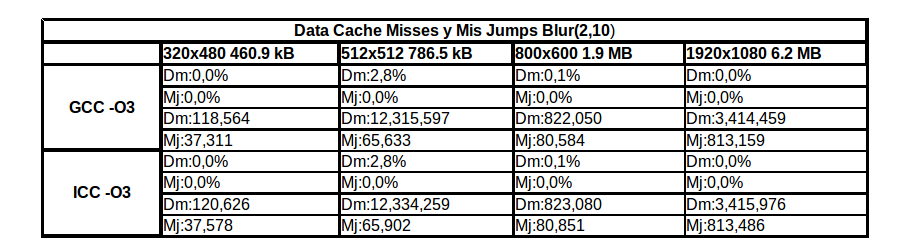
\includegraphics[width=\linewidth]{cachecompiladores/blur15.png}
%\endminipage
\end{center}
\end{figure}


\begin{figure}[H]
\begin{center}
%\minipage{0.8\textwidth}
  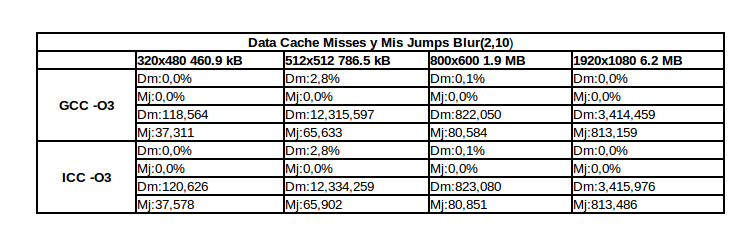
\includegraphics[width=\linewidth]{cachecompiladores/blur210cache.png}
%\endminipage
\end{center}
\end{figure}

\subsection{Conclusiones:}
En estas últimas imágenes podemos observar un manejo muy similar por parte de ambos compiladores. Si bien los valores pueden diferir un poco, al final del día, el porcentaje es igual.\\
Con los experimentos realizados anteriormente y los experimentos detallados en una sección anterior podemos llegar a la conclusión de que los compiladores ICC y GCC sin importar si la optimización \textit{-O3} está activa o no, manejan la caché de manera similar y podemos concluir que si ICC le gana a GCC en cuanto a velocidad eso no se debe a un mejor uso de la caché.\\
Antes habiamos visto una mayor velocidad con los filtros compilados con ICC. Aquí podemos confirmar que eso no se debe a un mejor uso de la caché.
